\begin{block}{Parameter Identification}
\centering
        \heading{Goal: Obtain the Best Value of $\lambda$} 
            {\large \textbf{Bayesian Context:} Simple Bayes model uses assumed likelihood function of data given $\lambda$.}
            
            {\large \textbf{Data Consistent Context:} Uses data to construct a predicted distribution of the average residuals given $\lambda$.}
            
            {\large How do we update initial descriptions of uncertainty using model predictions and data?}

        %\heading{Background}
             %{\large \emph{Data Consistent Inversion} is a Measure-Theoretic Framework for the solution of stochastic inverse problems. }
             %{\large \textbf{Data-Consistent Inversion} is a novel framework that uses push-forward and pull-back measures to ensure solutions are consistent with the observed distribution of data.}

        %\heading{Question} 
          %   {\large \emph{How do we cast a \textbf{Parameter Identification} problem in the context of Data-Consistent Inversion?} }

\end{block}


\begin{block}{Example}
\centering
    Consider an exponential decay problem with uncertain initial condition:
%    \begin{equation*}
%        \partial_t u = - u, \; u(t_0) = \lambda^\dagger = 0.5
%    \end{equation*}
\vspace{-0.5cm}
    \begin{figure}
        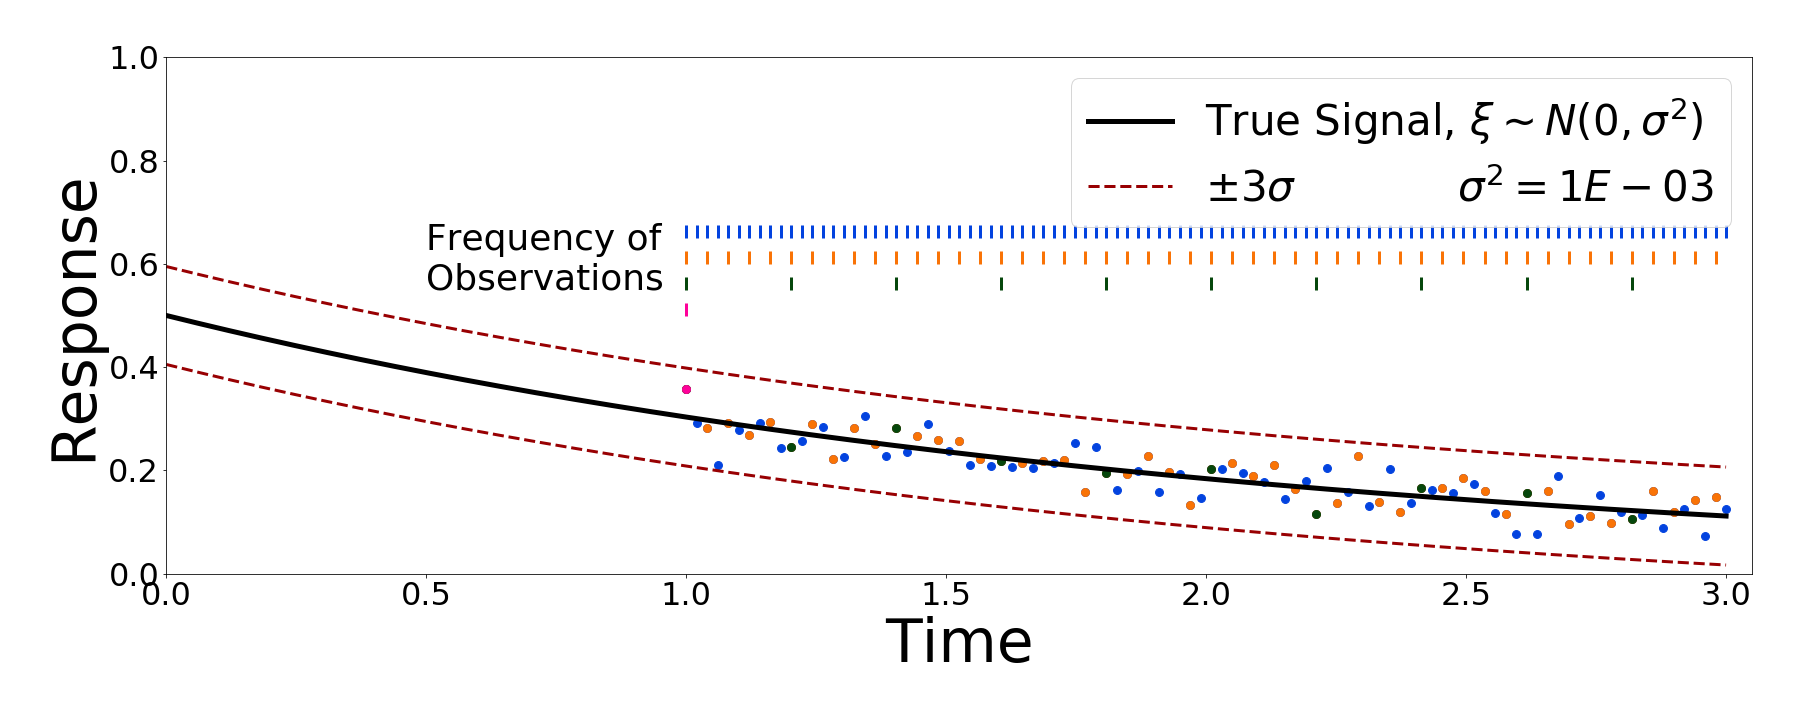
\includegraphics[width=26cm]{figures/exponential_decay_response_sigma-10E-4}
    \end{figure}

%\end{block}

\vspace{1cm}

%\begin{block}{Convergence}
\centering
\heading{\LARGE Convergence}
{\emph How do solutions change with more data?}
\vspace{-0.5cm}
    \begin{figure}
        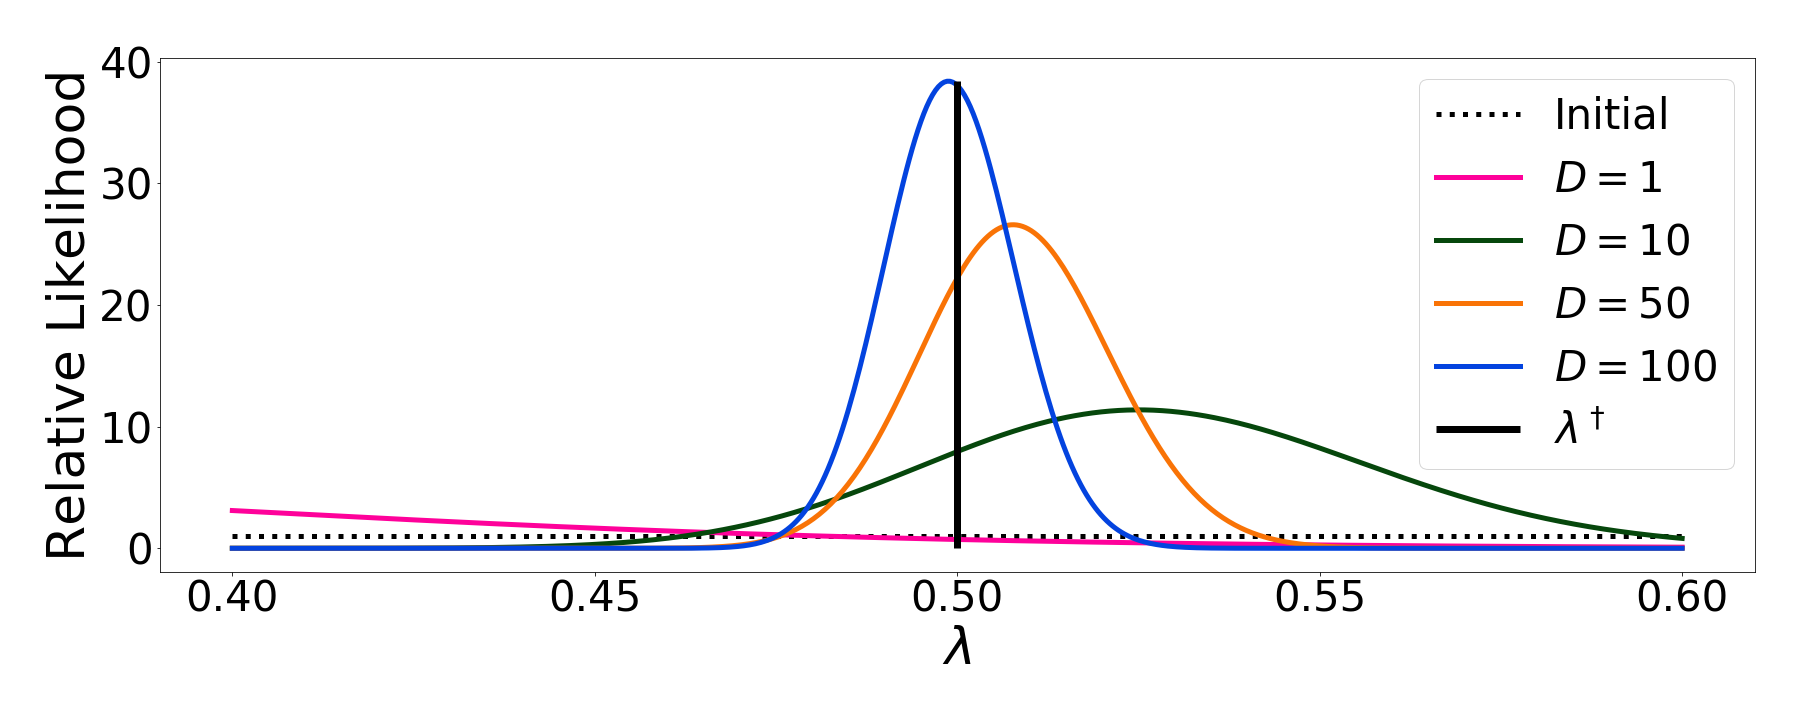
\includegraphics[width=26cm]{figures/updated_convergence_sigma-10E-4}
        \vspace{-0.5cm}
        \caption{ $\param^\dagger$ and $\updated$ for $D=1, 10, 50, 100$ for $N=1000$}
    \end{figure}

%\end{block}

\vspace{1cm}

%\begin{block}{Stability}
\heading{\LARGE Stability}
{\emph How do solutions on conditionals of $\nspace$ compare?}
\vspace{-0.5cm}
    \begin{figure}
        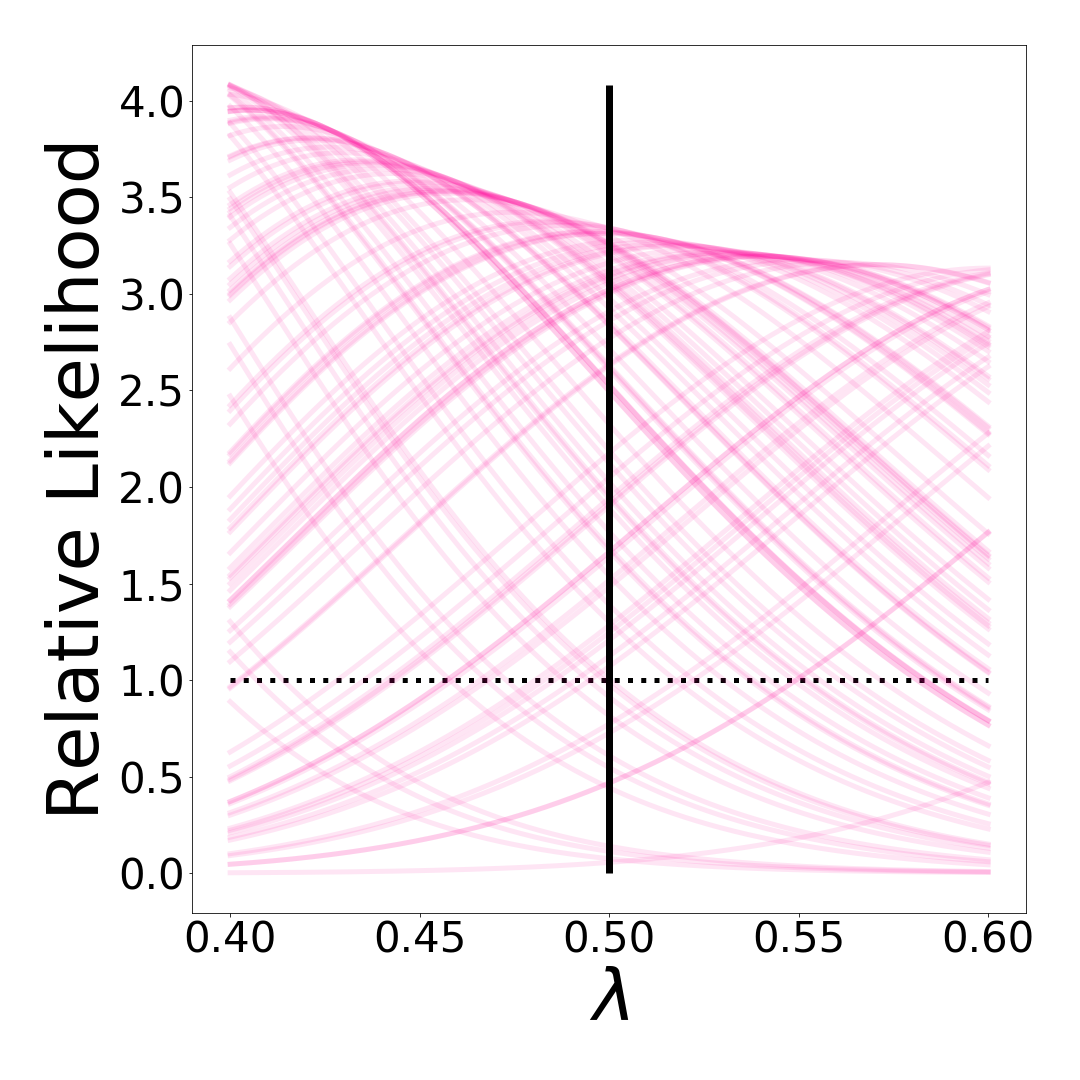
\includegraphics[width=13cm]{figures/updated_stability_D1_sigma-10E-4}
        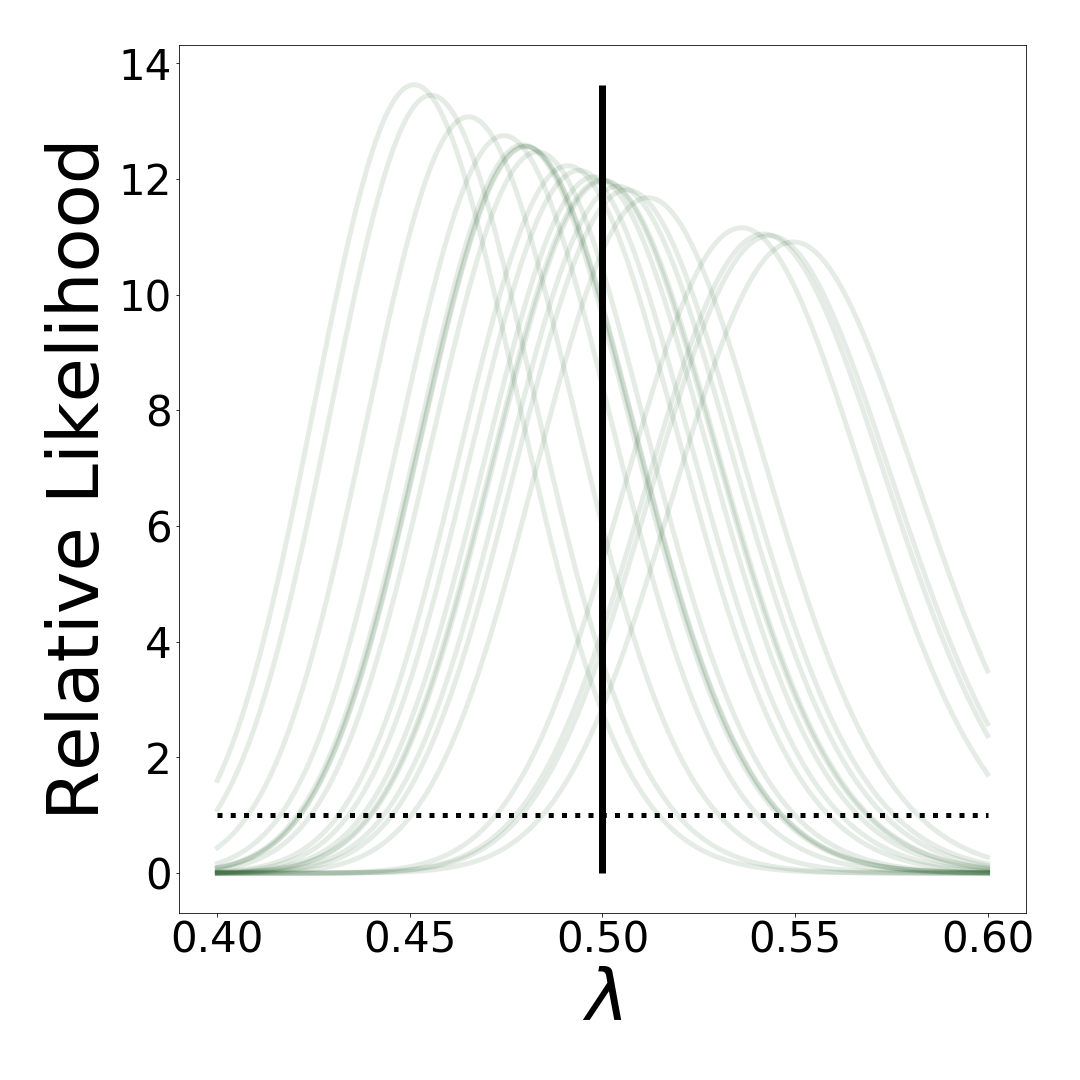
\includegraphics[width=13cm]{figures/updated_stability_D10_sigma-10E-4}\\
        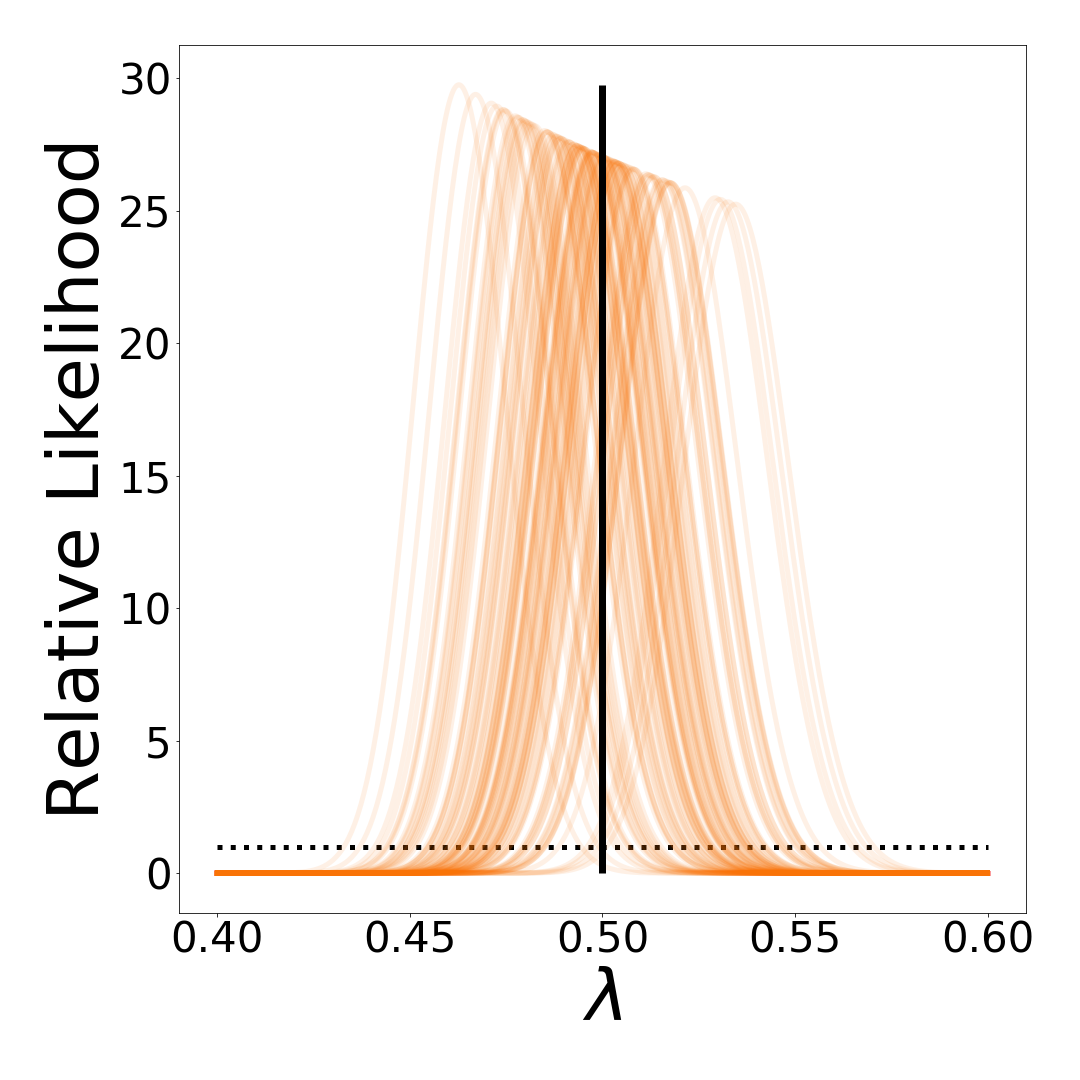
\includegraphics[width=13cm]{figures/updated_stability_D50_sigma-10E-4}
        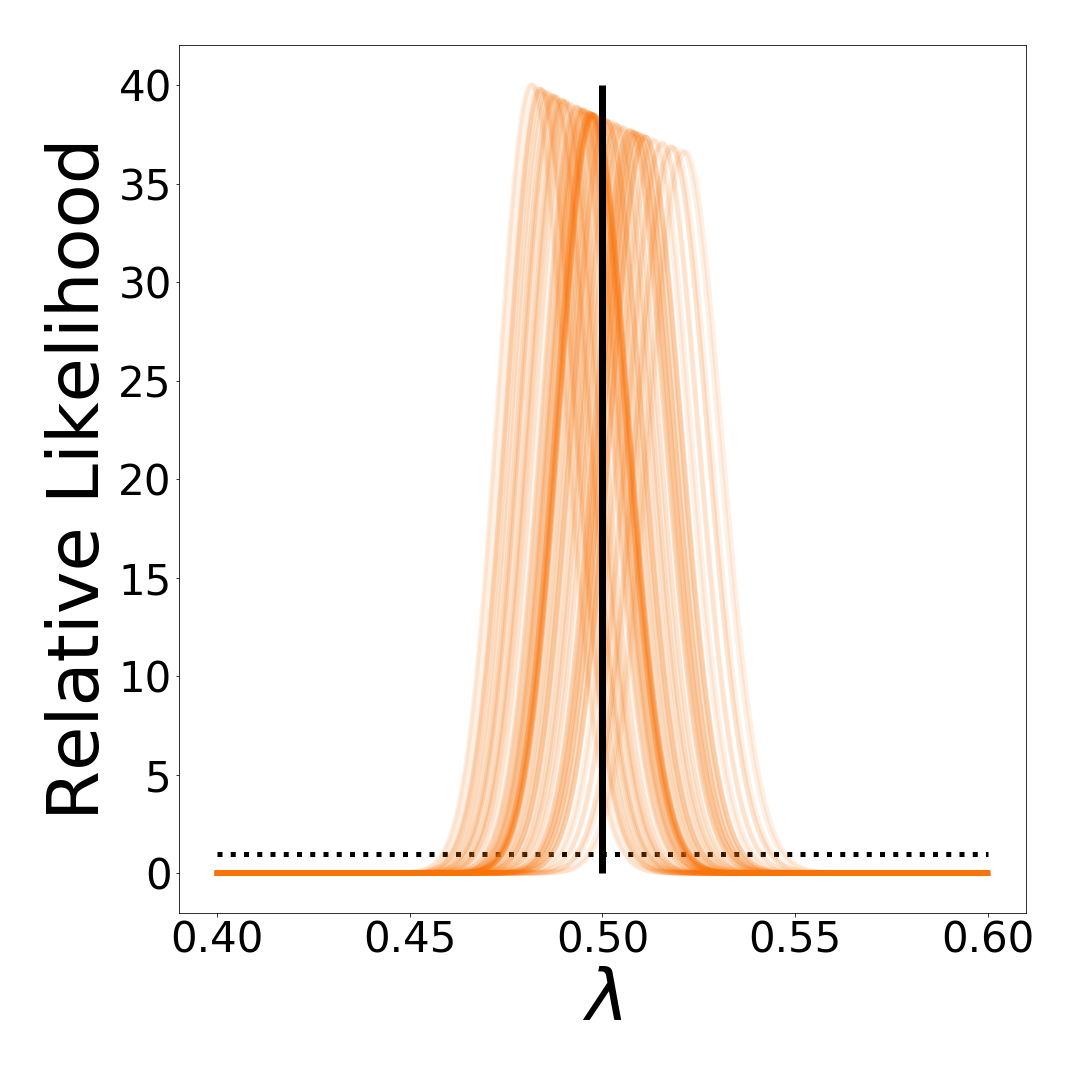
\includegraphics[width=13cm]{figures/updated_stability_D100_sigma-10E-4}
        \vspace{-1cm}
        \caption{$\param^\dagger$ and $\updated$ for one hundred realizations of $\noise^\dagger$ for $D=1, 10, 50, 100$}
    \end{figure}

\end{block}
